\documentclass[11pt,a4paper]{article}
\usepackage[T1]{fontenc}
\usepackage[utf8]{inputenc}
\usepackage{lmodern}
\usepackage{microtype}
\usepackage[margin=2.6cm]{geometry}
\usepackage{amsmath,amssymb}
\usepackage{booktabs}
\usepackage{graphicx}
\usepackage{caption}
\usepackage{float}
\usepackage{enumitem}
\usepackage[round,authoryear]{natbib}
\usepackage[hidelinks]{hyperref}
\newcommand{\metagenerated}{2026-10-23}
\newcommand{\metasha}{722acc1c6d}
\newcommand{\metaconfighash}{be08cae43cee}
\newcommand{\metanrows}{190,787}
\newcommand{\metanfeatures}{43}
\newcommand{\metadatastart}{2010-04-06}
\newcommand{\metadataend}{2026-09-30}
\newcommand{\metantickers}{46}
\newcommand{\metavnumpy}{2.4.6}
\newcommand{\metavpandas}{3.1.0}
\newcommand{\metavscikitlearn}{1.9.1}
\newcommand{\metavlightgbm}{4.7.0}
\newcommand{\metavstatsmodels}{0.15.0}
\newcommand{\metavtorch}{2.14.1}
\newcommand{\metavyfinance}{1.7.0}
\newcommand{\metavpython}{3.11.16}

\captionsetup{font=small,labelfont=bf,width=.92\textwidth}
\setlength{\parskip}{3pt}
\newcommand{\task}[1]{\texttt{#1}}
\newcommand{\E}{\mathbb{E}}
\DeclareMathOperator{\sign}{sign}
\DeclareMathOperator{\rank}{rank}
% shrink a table to the text width only when it is wider
\newsavebox{\tablebox}
\newcommand{\fitwidth}[1]{\sbox{\tablebox}{#1}\ifdim\wd\tablebox>\textwidth\resizebox{\textwidth}{!}{\usebox{\tablebox}}\else\usebox{\tablebox}\fi}

\title{Do Transformers Add Predictive Value for Short-Horizon Equity Forecasting?\\
\large A leak-free walk-forward benchmark against linear, gradient-boosted and recurrent baselines}
\author{\texttt{stockbench} working paper\\
\small Experiment \texttt{exp02}, configuration \texttt{\metaconfighash}, code revision \texttt{\metasha}}
\date{\metagenerated}

\begin{document}
\maketitle

\begin{abstract}
We ask whether a transformer encoder improves on strong, cheap baselines for three canonical short-horizon prediction problems on daily US equity data: the log realised volatility of the next five trading days, the sign of the next five-day return, and the cross-sectional rank of that return within a 46-name universe. A naive forecast, ridge or logistic regression, LightGBM, a two-layer LSTM and a channel-independent PatchTST encoder are trained on identical features and evaluated on an identical rolling walk-forward design with 60-month training, 6-month validation and 12-month test blocks, a horizon purge at every block boundary, and scalers fitted on training rows only. Eleven out-of-sample years (2015-07 to 2026-07, \metanrows{} samples) are scored with task-appropriate metrics, Diebold--Mariano tests against both the naive forecast and LightGBM using a Newey--West variance, three seeds per neural model, and a costed long/short backtest. On volatility every model beats the random walk by a wide margin, ridge regression is the best model (RMSE 0.495 against 0.634 naive and 0.508 LightGBM), and PatchTST is statistically indistinguishable from LightGBM (0.510; DM $+0.7$). Direction and rank are null results for every model: no model beats the base rate on direction, and the only ranking signal with a $t$-statistic above two (LSTM, rank IC 0.019) is too small to trade. Net of 10 basis points per side, every long/short decile book loses money while buy-and-hold SPY compounds at 14\% a year; annual turnover of 100 to 150 units of capital costs 10 to 15 percentage points of return and nothing in the model set has a gross edge large enough to pay for it. The transformer therefore adds no predictive value in this setting, and the harness that establishes this, with its leakage tests and resumable fit cache, is released with the paper.
\end{abstract}

\section{Introduction}

Transformer architectures \citep{vaswani2017attention} dominate sequence modelling in language and vision, and a growing literature applies them to time-series forecasting, with PatchTST \citep{nie2023patchtst} and the Temporal Fusion Transformer \citep{lim2021tft} among the most cited designs. Whether this capacity transfers to financial return prediction is an open question. Financial series have a signal-to-noise ratio that is orders of magnitude lower than the electricity, traffic and weather benchmarks on which long-horizon forecasting transformers are usually evaluated, and even in those benchmarks a single linear layer has been shown to be competitive \citep{zeng2023transformers}. At the same time, the machine-learning asset-pricing literature reports that flexible models do extract a small but economically meaningful premium from large cross-sections of monthly characteristics \citep{gu2020empirical}, so the question cannot be settled by appeal to efficiency alone \citep{fama1970efficient}.

This paper addresses the question with a benchmark rather than a new model. We fix a modest universe of liquid US equities, three prediction targets at a five-trading-day horizon, a feature set that every model sees in exactly the same form, and a rolling walk-forward evaluation with explicit guards against lookahead. Into this harness we place five models of increasing capacity: a naive forecast, a penalised linear model, gradient-boosted trees, a small LSTM \citep{hochreiter1997lstm}, and a PatchTST-style encoder. The design question is not whether a transformer can fit financial data, which it trivially can, but whether, under identical information and an identical test protocol, it predicts better than cheaper models by a margin that survives a formal test of predictive accuracy \citep{diebold1995comparing} and the transaction costs of acting on the forecast.

The contributions are threefold. First, we document an evaluation protocol in which every potential channel of leakage is closed by construction and verified by test: features use only data at or before the sample date, every training and validation target is realised before the test block opens, the sequence models' lookback windows cannot cross a block boundary in the forward direction, and all standardisation is estimated on training rows alone. Second, we report a complete comparison on eleven out-of-sample years with uncertainty from both fold-to-fold variation and seed-to-seed variation, with Diebold--Mariano statistics against two baselines, and with a backtest that charges realistic costs. Third, we obtain a clean null result: the transformer is never better than LightGBM at any conventional significance level, is dominated by ridge regression on the one target where any model has skill, and produces no tradable signal on the two directional targets. A defensible null was an explicit acceptance criterion of the study, and the harness is built so that a future model can be dropped in without changing the protocol.

The remainder of the paper is organised as follows. Section~\ref{sec:related} places the study in the literature. Section~\ref{sec:data} describes the data and Section~\ref{sec:method} the targets, features, walk-forward design, models and statistical tests. Section~\ref{sec:results} reports the results, Section~\ref{sec:discussion} interprets them, Section~\ref{sec:limitations} lists the limitations and Section~\ref{sec:conclusion} concludes. The appendix lists the universe, per-fold results and the reproduction commands.

\section{Related work}\label{sec:related}

\paragraph{Machine learning in asset pricing.} \citet{gu2020empirical} compare linear, tree and neural methods on a monthly panel of roughly 30{,}000 US stocks and 94 characteristics and find that neural networks and boosted trees deliver out-of-sample $R^2$ of the order of 0.3 to 0.4 per cent for individual stock returns, with the gains concentrated in nonlinear interactions among a handful of price-trend characteristics. \citet{israel2020can} argue that the small sample of independent observations, the low signal-to-noise ratio and the evolving nature of markets make finance an unusually hard domain for machine learning and that gains must be evaluated against the strongest simple benchmarks. Our setting is deliberately narrower (46 names, daily data, a five-day horizon, technical features only) and is closer to the practitioner question of whether a sequence model earns its cost on a small liquid book.

\paragraph{Transformers for time series.} PatchTST \citep{nie2023patchtst} segments each univariate series into overlapping patches, embeds each patch as a token, processes the channels independently with a shared encoder and reads the forecast from a flattened representation; it set the state of the art on the standard long-horizon benchmarks at the time of publication. \citet{zeng2023transformers} showed that a one-layer linear model matches or beats several earlier transformer designs on the same benchmarks, which motivated the patching and channel-independence of PatchTST and also motivates our inclusion of a linear baseline on exactly the same information. The Temporal Fusion Transformer \citep{lim2021tft} adds variable selection and static covariates; it is out of scope here but the harness admits it.

\paragraph{Volatility forecasting.} Realised volatility is strongly persistent and well described by simple autoregressive structure \citep{andersen2003modeling,corsi2009simple}, and \citet{hansen2005forecast} found that few models beat a GARCH(1,1) out of sample. Comparing volatility forecasts requires a loss that is robust to the noise in the realised proxy; \citet{patton2011volatility} shows that squared error and QLIKE are the two members of the robust family, and we report both.

\paragraph{Evaluation and overfitting.} The Diebold--Mariano test \citep{diebold1995comparing} with a heteroskedasticity- and autocorrelation-consistent variance \citep{newey1987simple} is the standard tool for comparing forecast accuracy on dependent series. \citet{bergmeir2012use} and \citet{lopezdeprado2018advances} discuss why ordinary cross-validation misstates the accuracy of time-series learners and why a purge between training and test observations is necessary when targets span several periods. \citet{bailey2014pseudo} and \citet{harvey2016cross} quantify the extent to which model selection on a backtest inflates reported performance; we respond by fixing the model set and the hyperparameter grids before any test fold is scored and by reporting every configuration that was run. \citet{novymarx2016taxonomy} document that transaction costs eliminate most of the apparent profits of high-turnover anomalies, which is the central finding of our backtest as well.

\section{Data}\label{sec:data}

\subsection{Universe and sources}

The universe is 45 large-capitalisation US equities with continuous daily history since January 2010, listed in Appendix~\ref{app:universe}, plus the SPDR S\&P 500 ETF (SPY), for \metantickers{} tradable names. Daily open, high, low, close, adjusted close and volume are retrieved from Yahoo Finance through the \texttt{yfinance} package (version \metavyfinance), with dividends and splits applied through the adjusted close. Four cross-asset series are retrieved on the same calendar and used only as features: SPY itself, the CBOE volatility index (\texttt{\^{}VIX}), the US dollar index (\texttt{DX-Y.NYB}) and the ten-year Treasury yield (\texttt{\^{}TNX}). Cross-asset series are aligned to SPY's trading calendar and forward-filled, so a missing print never pulls information from a later date. Raw bars are cached locally as one Parquet file per ticker; the loader is a plain callable so that a different vendor can be substituted without touching the rest of the pipeline.

The sample runs from \metadatastart{} (the first date at which every feature's longest window is complete) to \metadataend{} and contains \metanrows{} ticker-day observations with \metanfeatures{} features each. The panel is balanced apart from a small number of exchange holidays that differ across the cross-asset series.

\subsection{Survivorship}

The universe was chosen in 2026 from names that are large and liquid today and have a full history. It therefore excludes every firm that was delisted, acquired or shrank out of the large-cap set between 2010 and 2026, and it includes names such as NVDA and LLY whose rise is known only in hindsight. The bias affects all five models identically, so it does not change the comparison among them, but it inflates the unconditional upward drift of the panel (and hence the base rate that the naive direction model exploits), flatters the SPY benchmark and every long/short book alike, and means that the absolute numbers should not be read as estimates of what a point-in-time universe would have delivered \citep{shumway1997delisting}.

\subsection{Walk-forward folds}

Table~\ref{tab:folds} lists the eleven folds. All blocks are half-open calendar intervals. Fold $k$ trains on $[2010\text{-}01\text{-}01 + k\,\text{y},\ 2015\text{-}01\text{-}01 + k\,\text{y})$, validates on the following six months and tests on the following twelve; a fold is kept only if its test block is completely observed. Sample counts differ slightly across folds because of the purge described in Section~\ref{sec:walkforward} and because the direction target discards samples inside its dead zone (last column).

\begin{table}[H]
\centering\small
\caption{Walk-forward folds. $n$ counts ticker-day samples after purging; $n_{\text{test}}^{\text{dir}}$ is the number of test samples that carry a direction label.}
\label{tab:folds}
\begin{tabular}{lllllrrrr}
\toprule
$k$ & Train start & Val.\ start & Test start & Test end & $n_{\text{train}}$ & $n_{\text{val}}$ & $n_{\text{test}}$ & $n_{\text{test}}^{\text{dir}}$ \\
\midrule
0 & 2010-01-01 & 2015-01-01 & 2015-07-01 & 2016-07-01 & 54,740 & 5,453 & 11,638 & 10,803 \\
1 & 2011-01-01 & 2016-01-01 & 2016-07-01 & 2017-07-01 & 57,617 & 5,520 & 11,592 & 10,280 \\
2 & 2012-01-01 & 2017-01-01 & 2017-07-01 & 2018-07-01 & 57,617 & 5,520 & 11,546 & 10,546 \\
3 & 2013-01-01 & 2018-01-01 & 2018-07-01 & 2019-07-01 & 57,663 & 5,520 & 11,500 & 10,676 \\
4 & 2014-01-01 & 2019-01-01 & 2019-07-01 & 2020-07-01 & 57,617 & 5,474 & 11,638 & 10,840 \\
5 & 2015-01-01 & 2020-01-01 & 2020-07-01 & 2021-07-01 & 57,617 & 5,520 & 11,592 & 10,769 \\
6 & 2016-01-01 & 2021-01-01 & 2021-07-01 & 2022-07-01 & 57,684 & 5,474 & 11,592 & 10,868 \\
7 & 2017-01-01 & 2022-01-01 & 2022-07-01 & 2023-07-01 & 57,684 & 5,474 & 11,546 & 10,877 \\
8 & 2018-01-01 & 2023-01-01 & 2023-07-01 & 2024-07-01 & 57,684 & 5,474 & 11,500 & 10,690 \\
9 & 2019-01-01 & 2024-01-01 & 2024-07-01 & 2025-07-01 & 57,638 & 5,474 & 11,500 & 10,831 \\
10 & 2020-01-01 & 2025-01-01 & 2025-07-01 & 2026-07-01 & 57,638 & 5,382 & 11,546 & 10,895 \\
\bottomrule
\end{tabular}

\end{table}

\section{Methodology}\label{sec:method}

\subsection{Targets}

Let $P_{i,t}$ be the adjusted close of name $i$ on trading day $t$, $p_{i,t}=\log P_{i,t}$, and $r_{i,t}=p_{i,t}-p_{i,t-1}$ the one-day log return. With horizon $H=5$ trading days, the forward return is $f_{i,t}=p_{i,t+H}-p_{i,t}$ and the three targets are
\begin{align}
y^{\text{vol}}_{i,t} &= \log\sqrt{\tfrac{1}{H}\textstyle\sum_{j=1}^{H} r_{i,t+j}^{2}}, \label{eq:vol}\\
y^{\text{dir}}_{i,t} &= \mathbf{1}\{f_{i,t}>0\}\quad\text{defined only when } |f_{i,t}|\ge\delta,\ \delta=0.25\%, \label{eq:dir}\\
y^{\text{rank}}_{i,t} &= \frac{\rank_{i'\in\mathcal{U}_t}\!\big(f_{i',t}\big)(i)}{|\mathcal{U}_t|}\in(0,1], \label{eq:rank}
\end{align}
where $\mathcal{U}_t$ is the set of names with a forward return on day $t$. The volatility target is the log of the realised standard deviation of daily returns over the next five bars, so that squared error on it is a relative error on volatility. The direction target drops the 8 to 11 per cent of samples whose five-day move is inside $\pm 0.25\%$, which removes the observations whose sign is indistinguishable from noise. The rank target is a cross-sectional percentile, so it is invariant to the market return on the day and asks only for relative ordering.

Every target depends on bars $t+1,\dots,t+H$. We record for every sample the date of bar $t+H$ as its \emph{target end}, and because the rank target couples all names on a date, we define the target end of a date as the latest target end among its names. This quantity drives the purge.

\subsection{Features}\label{sec:features}

Every model sees the same \metanfeatures{} features, computed per name from data at or before $t$ and registered in a single table so that a new feature is one function. Per name: cumulative log returns $p_{t}-p_{t-k}$ for $k\in\{1,2,3,5,10,21\}$; realised volatility $\log\sqrt{\tfrac{1}{w}\sum_{j=0}^{w-1}r_{t-j}^2}$ for $w\in\{5,21,63\}$, so that the five-bar version is the lagged analogue of the target in \eqref{eq:vol}; a volume $z$-score, the log volume against its trailing 21-bar mean and standard deviation; the 14-day relative strength index with Wilder's exponential smoothing \citep{wilder1978new}; the MACD, the difference between 12- and 26-day exponential moving averages divided by the close, and its 9-day signal-line histogram; and the maximum drawdown over the trailing 21 bars. Cross-asset: SPY log returns at 1, 5 and 21 bars and its 21-bar realised volatility; the log VIX level and its 1- and 5-bar changes; 1- and 5-bar changes in the dollar index and the ten-year yield. Calendar: five day-of-week and twelve month-of-year indicators. Rows with any undefined feature (the warm-up at the start of each series) are dropped once for all tasks; rows with an undefined target are dropped per task.

\subsection{Walk-forward design and leakage control}\label{sec:walkforward}

The evaluation is a rolling walk-forward with calendar blocks (Table~\ref{tab:folds}). For fold $k$ with validation start $v_k$, test start $s_k$ and test end $e_k$, a sample $(i,t)$ belongs to the training set if $t$ lies in the training block \emph{and} its target end is before $v_k$; to the validation set if $t$ lies in the validation block and its target end is before $s_k$; and to the test set if $s_k\le t<e_k$. The two ``target end'' conditions implement the purge of \citet{lopezdeprado2018advances}: no training or validation label is computed from a bar that belongs to a later block, so the model never sees, even partially, a return that it will be asked to predict. The purge removes the last five trading days of every training and validation block.

Feature scalers, the target standardisation used by the neural models, the penalty of the linear model, the number of boosting rounds and the early-stopping epoch of the neural models are all determined from the training and validation sets of the fold alone. The test block is scored exactly once per model and seed; no quantity estimated on it feeds back into any model.

The sequence models consume, for sample $(i,t)$, the window of the last $L=64$ feature vectors of name $i$ ending at $t$. Windows are materialised as a zero-copy strided view over a ticker-major array, so that a window can never straddle two names. A training or validation window ending at $t$ contains only bars at or before $t$, and since $t$ precedes the next block, the window cannot reach forward into it. A test window may reach back into the validation or training period, which is the information a live model would have; this is the asymmetric convention and is stated here because the alternative (dropping the first 63 test days of each fold) would discard a quarter of the test sample for no gain in validity. Samples that lack a full window (the first 63 bars of each name in 2010) are excluded from the sequence models' training set only.

These properties are enforced by tests that run before any model is fitted. The feature test perturbs every bar after a cutoff date with a large shock and asserts bit-for-bit equality of every feature before the cutoff. The target test counts the samples whose target window straddles the cutoff and asserts that only those change. The split test asserts that no training or validation sample of any fold has a target end inside any test block and that no test date is scored by more than one fold. The window test asserts that every window equals the rows $t-L+1,\dots,t$ of the same name and that exactly $(L-1)$ rows per name lack a window. The linear model's scaler is checked to reproduce the training-row mean and variance.

\subsection{Models}

All models receive the same training, validation and test rows of a fold. The gradient-boosted and neural models use the validation block for early stopping; the linear model uses it to choose its penalty; the naive model ignores it.

\paragraph{Naive.} For volatility, the random-walk forecast $\hat y_{i,t}=\log\sqrt{\tfrac{1}{5}\sum_{j=0}^{4}r_{i,t-j}^2}$, that is, the last five-bar realised volatility (the feature \texttt{rv\_5}). For direction, the training-set frequency of the positive class, a constant probability. For rank, the training-set mean of the target, a constant that equals $0.5$ up to rounding.

\paragraph{Ridge and logistic regression.} A \texttt{StandardScaler} fitted on training rows followed by ridge regression (volatility and rank) or $\ell_2$-penalised logistic regression (direction). The penalty is parameterised on the per-sample scale, $\alpha=\lambda n$ for ridge and $C=1/(\lambda n)$ for logistic regression with $n$ the number of training rows, and $\lambda$ is chosen from $\{10^{-4},10^{-3},10^{-2},10^{-1},1\}$ by squared error (Brier score for direction) on the validation block.

\paragraph{LightGBM.} Gradient-boosted trees \citep{ke2017lightgbm} with up to 2{,}000 rounds at learning rate 0.02, 31 leaves, a minimum of 100 samples per leaf, row and column subsampling of 0.8, $\ell_2$ regularisation of 1.0, deterministic row-wise histograms, and early stopping on the validation loss with a patience of 100 rounds. The best iteration is recorded; when it is one, the model has reduced to a constant close to the training mean.

\paragraph{LSTM.} Two stacked LSTM layers of 64 units with dropout 0.2 between the layers and before a linear head that reads the final hidden state \citep{hochreiter1997lstm}.

\paragraph{PatchTST.} A channel-independent encoder in the design of \citet{nie2023patchtst}. Each of the \metanfeatures{} feature channels of a 64-bar window is cut into 15 patches of length 8 with stride 4, each patch is linearly embedded into $d_{\text{model}}=64$ dimensions and given a learned positional embedding, and the sequence of patches is processed by two pre-norm transformer encoder layers with four heads, a feed-forward width of 128, GELU activations and dropout 0.3, followed by a final layer normalisation. Encoder weights are shared across channels. A shared flatten head maps the $15\times 64$ encoded patches of a channel to one scalar, and a linear channel mixer maps the \metanfeatures{} channel scalars to the prediction. We omit the reversible instance normalisation of the original design because the level of the inputs, for instance the current realised volatility, is signal in this problem rather than nuisance. The model has about 60{,}000 parameters.

\paragraph{Neural training.} Inputs are standardised with training-row statistics and clipped to $\pm 5$; regression targets are standardised with training-row statistics and classification uses the logit with a binary cross-entropy loss. Adam \citep{kingma2015adam} with learning rate $10^{-3}$, batches of 512 windows, gradient-norm clipping at 1.0, at most 20 epochs, and early stopping on the validation loss with a patience of 3 epochs and restoration of the best epoch's weights. Each fit is run for seeds $\{0,1,2\}$, which fix initialisation, batch order and dropout masks. Training runs on an Apple M5 GPU through the Metal backend; repeated fits on this device reproduced predictions bit for bit, although the framework does not guarantee it.

\subsection{Metrics}

For volatility we report the root mean squared error and mean absolute error on the log-volatility scale and the QLIKE loss of \citet{patton2011volatility},
\begin{equation}
\text{QLIKE}=\frac{1}{n}\sum\Big(\frac{\sigma^2}{\hat\sigma^2}-\log\frac{\sigma^2}{\hat\sigma^2}-1\Big),\qquad \frac{\sigma^2}{\hat\sigma^2}=\exp\!\big(2(y-\hat y)\big).
\end{equation}
For direction we report accuracy, balanced accuracy and the area under the ROC curve, with the decision threshold at a predicted probability of $0.5$. For rank we report the information coefficient, the mean over test dates of the cross-sectional Pearson correlation between prediction and target, and the rank IC, its Spearman analogue, together with the $t$-statistic of the mean daily IC computed with a Newey--West variance at lag $H-1=4$. A constant prediction has an IC of exactly zero by convention.

All metrics are computed per fold and then summarised as the mean and standard deviation across the eleven folds; for the neural models the per-fold value is first averaged over seeds, and the standard deviation across seeds of the all-fold mean is reported separately as the seed uncertainty. ``Pooled'' values are computed on all test samples together.

\subsection{Diebold--Mariano tests}\label{sec:dm}

For models $A$ and $B$ with per-sample losses $\ell^A_{i,t}$ and $\ell^B_{i,t}$ (squared error for volatility and rank, the Brier score \citep{brier1950verification} for direction), define the daily loss differential
\begin{equation}
d_t=\frac{1}{|\mathcal{U}_t|}\sum_{i\in\mathcal{U}_t}\big(\ell^A_{i,t}-\ell^B_{i,t}\big)
\end{equation}
and the statistic $\text{DM}=\bar d/\sqrt{\hat V/T}$, where $\hat V$ is the Newey--West \citep{newey1987simple} long-run variance of $d_t$ with a Bartlett kernel truncated at lag $4$, the maximal overlap of two five-day targets \citep{diebold1995comparing}. Averaging across names before computing the variance removes the strong cross-sectional correlation of losses on a given day, which would otherwise understate the variance by a factor close to the number of names. A negative statistic means that $A$ has lower loss than $B$. We report the statistic for every model against the naive forecast and against LightGBM, pooled over all test dates and separately per fold; for the neural models we report the mean, minimum and maximum over seeds and the number of seeds significant at the 5\% level, and we count the (seed, fold) pairs significant at 5\% with the same sign as the pooled statistic. Direction tests use only the samples that carry a label. We apply no multiple-comparison correction; as every significant result in Section~\ref{sec:results} is in the direction of a baseline beating a more complex model, a correction would only strengthen the conclusions.

\subsection{Backtest}\label{sec:backtest}

The direction and rank predictions are traded with a simple long/short rule. On each test date $t$ the names are mid-ranked by their prediction, $\tilde\rho_{i,t}=(\rank(\hat y_{i,t})-\tfrac12)/|\mathcal{U}_t|$, and the book $w_{t}$ is equal-weight long the names with $\tilde\rho>0.9$ and equal-weight short the names with $\tilde\rho<0.1$, one dollar long and one dollar short per dollar of capital (five names per side in a 46-name universe). Ties share the average rank, so a constant prediction takes no positions rather than arbitrary ones. A book formed at the close of $t$ earns the daily simple returns $R_{i,t+1},\dots,R_{i,t+H}$. With one book formed every day, capital is split equally across the $H$ live books, so the weights held through day $d$ are the calendar-time average of \citet{jegadeesh1993returns},
\begin{equation}
W_{d}=\frac{1}{H}\sum_{j=1}^{H} w_{d-j},\qquad
r^{\text{gross}}_{d}=\sum_i W_{d,i}R_{i,d},\qquad
r^{\text{net}}_{d}=r^{\text{gross}}_{d}-c\sum_i\big|W_{d,i}-W_{d-1,i}\big|,
\end{equation}
with $c=10$ basis points per unit of notional traded. Weights are reset to target every day; drift inside a holding period is ignored. We report the geometric annualised return, the Sharpe ratio as $\sqrt{252}$ times the ratio of the mean to the standard deviation of daily returns with no risk-free adjustment \citep{lo2002statistics}, the maximum drawdown of the wealth path, the Newey--West $t$-statistic of the mean daily net return, and the annual turnover $\tfrac{252}{D}\sum_d\sum_i|W_{d,i}-W_{d-1,i}|$ in units of capital, for both gross and net returns. Buy-and-hold SPY over the same $2{,}769$ days with no costs is the benchmark. The neural models' seeds are backtested separately and summarised as mean and standard deviation.

Because the direction model drops samples inside the dead zone, the universe on which it is scored is a subset chosen with knowledge of the realised return. For the backtest the direction model therefore predicts on every test sample, labelled or not, and the dead zone is applied only when computing accuracy, AUC and the Diebold--Mariano statistics; otherwise the tradable universe on a date would consist of the names that, in hindsight, moved by more than 0.25\%.

\section{Results}\label{sec:results}

\subsection{Volatility}

\begin{table}[H]
\centering\scriptsize
\caption{Five-day log realised volatility. Mean $\pm$ standard deviation across the eleven test folds, seed-averaged per fold; ``Seed sd'' is the standard deviation across seeds of the all-fold mean RMSE. DM statistics are pooled over all test dates (negative: the row's model has lower loss than the baseline); for multi-seed models the mean and [min, max] over seeds. ``sig.'' counts (seed, fold) pairs significant at 5\% with the sign of the pooled statistic. $^{*}$, $^{**}$, $^{***}$: $p<0.10$, $0.05$, $0.01$.}
\label{tab:vol}
\fitwidth{\begin{tabular}{lrrrrrrrr}
\toprule
Model & RMSE & MAE & QLIKE & Seed sd & DM vs naive & sig. & DM vs LightGBM & sig. \\
\midrule
Naive & $0.634 \pm 0.035$ & $0.495 \pm 0.029$ & $1.443 \pm 0.250$ & -- & -- & -- & $+20.2^{***}$ & 10/11 \\
Ridge / logistic & $0.495 \pm 0.030$ & $0.384 \pm 0.025$ & $0.735 \pm 0.141$ & -- & $-31.7^{***}$ & 11/11 & $-3.7^{***}$ & 4/11 \\
LightGBM & $0.508 \pm 0.040$ & $0.393 \pm 0.031$ & $0.774 \pm 0.301$ & -- & $-20.2^{***}$ & 10/11 & -- & -- \\
LSTM (3 seeds) & $0.525 \pm 0.046$ & $0.409 \pm 0.037$ & $0.878 \pm 0.270$ & $0.005$ & $-17.0\ [-17.6,\ -16.2]$ & 30/33 & $+5.0\ [+4.0,\ +6.5]$ & 14/33 \\
PatchTST (3 seeds) & $0.510 \pm 0.051$ & $0.395 \pm 0.040$ & $0.854 \pm 0.368$ & $0.004$ & $-18.3\ [-20.4,\ -16.9]$ & 30/33 & $+0.7\ [-0.6,\ +2.0]$ & 4/33 \\
\bottomrule
\end{tabular}
}
\end{table}

\begin{figure}[H]
\centering
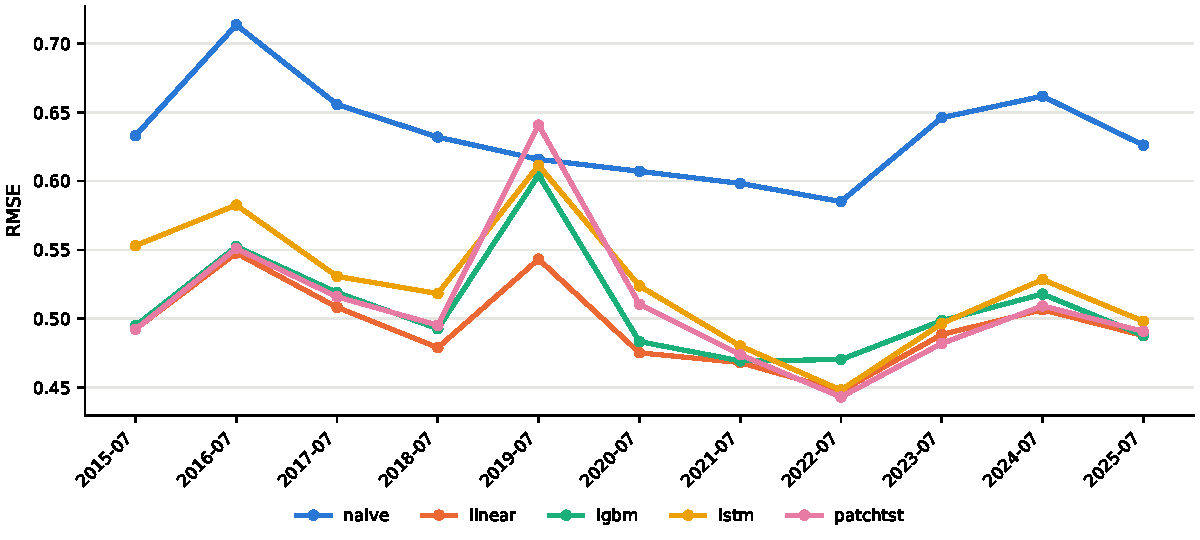
\includegraphics[width=\textwidth]{figures/fold_vol.pdf}
\caption{RMSE of the log realised volatility forecast by test fold, seed-averaged. The fold starting 2019-07 contains the March 2020 crash.}
\label{fig:fold_vol}
\end{figure}

Table~\ref{tab:vol} and Figure~\ref{fig:fold_vol} summarise the one target on which any model has skill. Every model beats the random walk in every fold, by a margin that the Diebold--Mariano test places far outside sampling variation (DM between $-17$ and $-32$ against naive; 30 to 33 of 33 seed-fold pairs significant for the neural models and 10 or 11 of 11 folds for the others). This is not surprising: five-day realised volatility is a noisy proxy, and any model that shrinks the last five-day estimate towards a longer-window level, as the 21- and 63-bar features allow, reduces its variance \citep{andersen2003modeling}. The ordering among the models is the informative part. Ridge regression on the \metanfeatures{} features has the lowest RMSE ($0.495$), MAE and QLIKE, and is significantly better than LightGBM in the pooled test (DM $-3.7$, $p<0.01$) although only in four of eleven folds individually. PatchTST is the second-best model by RMSE ($0.510$) and MAE and is statistically indistinguishable from LightGBM ($0.508$): the pooled DM statistic against LightGBM is $+0.7$ on average, ranges from $-0.65$ to $+2.05$ across seeds, and only one seed and four of 33 seed-fold pairs are significant. The LSTM ($0.525$) is significantly worse than LightGBM (DM $+5.0$ for every seed). Seed uncertainty is an order of magnitude smaller than fold uncertainty for both neural models (seed sd $0.004$ to $0.005$ against fold sd $0.046$ to $0.051$), so the ranking is not an artefact of initialisation.

Figure~\ref{fig:fold_vol} shows that the non-naive models move together across folds and that their worst year by far is the fold starting in July 2019, which contains the March 2020 crash: ridge degrades from about $0.49$ to $0.54$, LightGBM and the LSTM to $0.60$ to $0.61$, and PatchTST to $0.64$, worse than the random walk ($0.62$) in that fold. The regime break penalises the higher-capacity models more because their forecasts depend on a broader set of features whose relation to future volatility shifted. PatchTST beats ridge in three of the eleven folds (those starting 2015, 2022 and 2023) and loses in the other eight. On the robust QLIKE loss, which penalises under-prediction of variance more heavily, the gaps widen in the same order: ridge $0.735$, LightGBM $0.774$, PatchTST $0.854$, LSTM $0.878$, naive $1.443$.

\subsection{Direction}

\begin{table}[H]
\centering\scriptsize
\caption{Sign of the five-day return with a $\pm0.25\%$ dead zone. Layout as Table~\ref{tab:vol}; the naive model predicts the training-set frequency of the positive class and the DM loss is the Brier score.}
\label{tab:dir}
\fitwidth{\begin{tabular}{lrrrrrrrr}
\toprule
Model & Accuracy & Bal.\ acc. & AUC & Seed sd & DM vs naive & sig. & DM vs LightGBM & sig. \\
\midrule
Naive & $0.556 \pm 0.024$ & $0.500 \pm 0.000$ & $0.500 \pm 0.000$ & -- & -- & -- & $-1.4$ & 0/11 \\
Ridge / logistic & $0.553 \pm 0.026$ & $0.502 \pm 0.008$ & $0.509 \pm 0.029$ & -- & $+1.5$ & 0/11 & $+0.8$ & 0/11 \\
LightGBM & $0.556 \pm 0.024$ & $0.500 \pm 0.000$ & $0.507 \pm 0.016$ & -- & $+1.4$ & 0/11 & -- & -- \\
LSTM (3 seeds) & $0.511 \pm 0.038$ & $0.500 \pm 0.024$ & $0.507 \pm 0.029$ & $0.005$ & $+9.6\ [+8.7,\ +10.1]$ & 25/33 & $+9.8\ [+8.9,\ +10.2]$ & 25/33 \\
PatchTST (3 seeds) & $0.534 \pm 0.018$ & $0.496 \pm 0.010$ & $0.488 \pm 0.025$ & $0.006$ & $+5.7\ [+4.4,\ +6.7]$ & 16/33 & $+5.4\ [+4.1,\ +6.4]$ & 16/33 \\
\bottomrule
\end{tabular}
}
\end{table}

\begin{figure}[H]
\centering
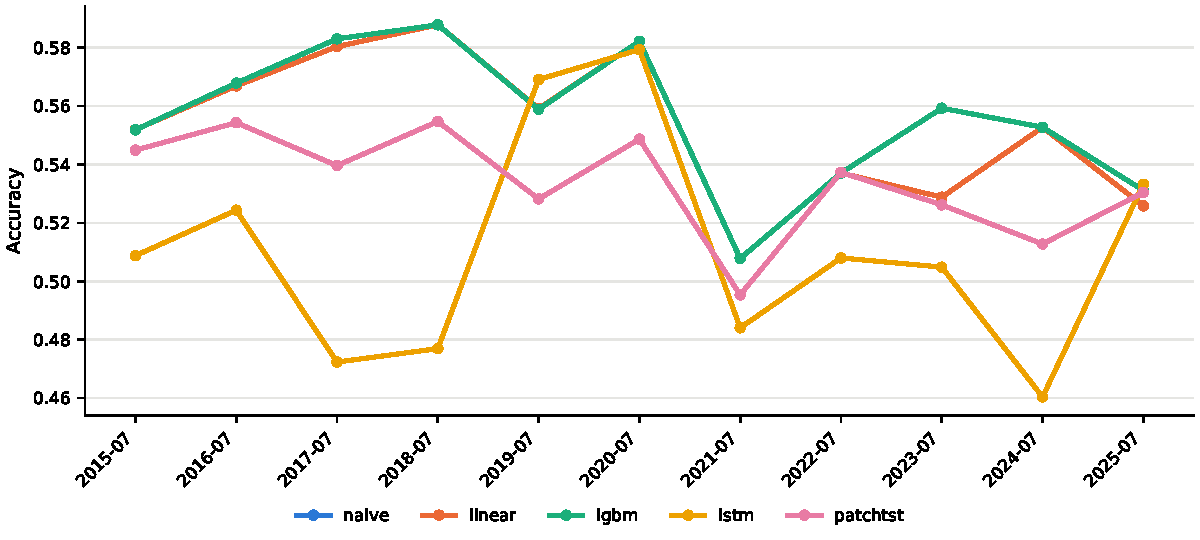
\includegraphics[width=\textwidth]{figures/fold_dir.pdf}
\caption{Accuracy of the direction forecast by test fold, seed-averaged. Naive and LightGBM overlap because LightGBM reduces to the base rate in most folds.}
\label{fig:fold_dir}
\end{figure}

Direction is a null result for every model (Table~\ref{tab:dir}, Figure~\ref{fig:fold_dir}). The naive model achieves $55.6\%$ accuracy because the labelled panel has an upward drift, and no model improves on it. Logistic regression reaches an AUC of $0.509$ and accuracy of $55.3\%$, LightGBM stops at its first boosting round in seven of eleven folds and therefore reproduces the base rate exactly; in the other four it stops within sixteen rounds and never assigns a probability below one half, so its accuracy equals the naive's in every fold. The pooled DM statistics of both against naive are positive and insignificant ($p=0.14$). The two neural models are significantly \emph{worse} than naive on Brier loss (LSTM DM $+9.6$, PatchTST $+5.7$, every seed significant) because they commit to both classes without having signal: the LSTM's accuracy is $51.1\%$ and PatchTST's $53.4\%$, both below the base rate, and PatchTST's AUC of $0.488$ is below one half. The training logs make the mechanism explicit. Early stopping selected the first epoch in 24 of the 33 PatchTST direction fits at a validation loss of about $0.69$ nats, which is the entropy of the base rate; the encoder found nothing to learn beyond the class frequency and its subsequent epochs only added variance.

\subsection{Cross-sectional rank}

\begin{table}[H]
\centering\scriptsize
\caption{Cross-sectional percentile rank of the five-day return. IC and rank IC are means over test dates of the daily cross-sectional Pearson and Spearman correlations; $t$-statistics use a Newey--West variance at lag 4 and are pooled over all test dates and averaged over seeds. DM losses are squared errors on the rank target.}
\label{tab:rank}
\fitwidth{\begin{tabular}{lrrrrrrrrr}
\toprule
Model & IC & Rank IC & Seed sd & $t$(IC) & $t$(Rank IC) & DM vs naive & sig. & DM vs LightGBM & sig. \\
\midrule
Naive & $0.000 \pm 0.000$ & $0.000 \pm 0.000$ & -- & $0.00$ & $0.00$ & -- & -- & $-2.1^{**}$ & 2/11 \\
Ridge / logistic & $0.012 \pm 0.026$ & $0.014 \pm 0.029$ & -- & $1.37$ & $1.64$ & $+0.4$ & 0/11 & $-1.5$ & 0/11 \\
LightGBM & $0.003 \pm 0.024$ & $0.005 \pm 0.027$ & -- & $0.40$ & $0.73$ & $+2.1^{**}$ & 2/11 & -- & -- \\
LSTM (3 seeds) & $0.020 \pm 0.042$ & $0.019 \pm 0.046$ & $0.005$ & $2.17$ & $2.12$ & $+4.9\ [+4.3,\ +5.8]$ & 14/33 & $+4.5\ [+3.9,\ +5.4]$ & 12/33 \\
PatchTST (3 seeds) & $0.002 \pm 0.028$ & $-0.001 \pm 0.028$ & $0.013$ & $0.23$ & $-0.16$ & $+2.5\ [+1.4,\ +3.1]$ & 7/33 & $+0.7\ [-0.5,\ +1.5]$ & 6/33 \\
\bottomrule
\end{tabular}
}
\end{table}

\begin{figure}[H]
\centering
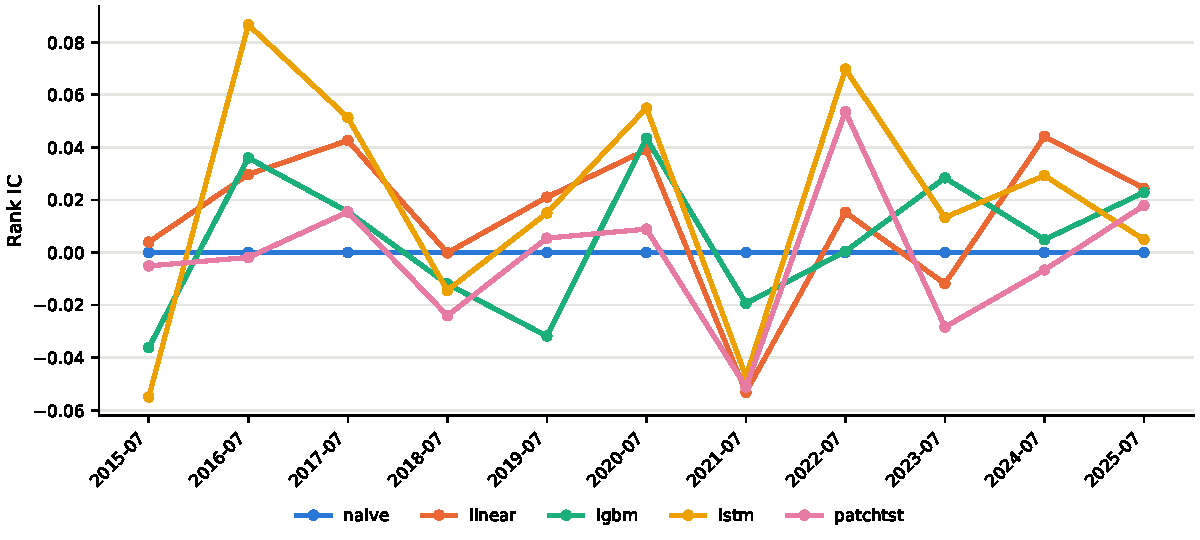
\includegraphics[width=\textwidth]{figures/fold_rank.pdf}
\caption{Rank IC by test fold, seed-averaged. The naive model predicts a constant and has an IC of exactly zero.}
\label{fig:fold_rank}
\end{figure}

No model produces a usable ranking signal (Table~\ref{tab:rank}, Figure~\ref{fig:fold_rank}). The LSTM has the highest IC and rank IC, $0.019$ and $0.019$, with pooled $t$-statistics of $2.2$ and $2.1$; ridge follows at $0.012$ and $0.014$ with $t$ of $1.4$ and $1.6$; LightGBM and PatchTST are indistinguishable from zero. For reference, a daily rank IC of $0.02$ on 46 names corresponds to an $R^2$ of $0.04\%$ for the cross-section and is well below the level at which decile portfolios overcome the costs of five-day rebalancing (Section~\ref{sec:bt_results}). The squared-error comparison is harsher still. Every model's mean squared error on the rank target is \emph{higher} than that of the constant predictor, significantly so for LightGBM (DM $+2.1$), PatchTST ($+2.5$, two of three seeds) and the LSTM ($+4.9$, all seeds): the models capture a trace of ordering but pay for it with calibration. PatchTST is also unstable across seeds on this target, with a seed standard deviation of its IC ($0.014$) three to four times that of the LSTM ($0.003$) and of the same order as its mean, which is itself a symptom of fitting noise. Figure~\ref{fig:fold_rank} shows every model's IC swinging between about $-0.05$ and $+0.09$ from year to year with no consistent sign and no model consistently above the others.

\subsection{Backtest}\label{sec:bt_results}

\begin{table}[H]
\centering\footnotesize
\caption{Long/short decile books formed from the direction predictions, five-day holding, 10 basis points per unit traded. Returns are geometric annualised; Sharpe ratios are on daily returns with no risk-free adjustment; $t$(net) is the Newey--West $t$-statistic of the mean daily net return; turnover is notional traded per year per unit of capital. Multi-seed models: mean $\pm$ standard deviation across seeds. ``--'': undefined because the strategy never trades.}
\label{tab:bt_dir}
\fitwidth{\begin{tabular}{lrrrrrrr}
\toprule
Model & Net return & Net Sharpe & Max DD & $t$(net) & Gross return & Gross Sharpe & Turnover \\
\midrule
Naive & $+0.0\%$ & -- & $0.0\%$ & $+0.00$ & $+0.0\%$ & -- & $0$ \\
Ridge / logistic & $-18.2\%$ & $-0.84$ & $-89.4\%$ & $-2.71$ & $-5.8\%$ & $-0.18$ & $141$ \\
LightGBM & $-3.0\%$ & $-0.14$ & $-40.7\%$ & $-0.59$ & $-2.3\%$ & $-0.09$ & $6$ \\
LSTM (3 seeds) & $-8.0\% \pm 2.7\%$ & $-0.24 \pm 0.12$ & $-68.3\% \pm 7.5\%$ & $-0.82 \pm 0.41$ & $+2.7\% \pm 3.0\%$ & $+0.23 \pm 0.13$ & $110 \pm 4$ \\
PatchTST (3 seeds) & $-12.0\% \pm 3.2\%$ & $-0.69 \pm 0.32$ & $-81.1\% \pm 4.4\%$ & $-2.32 \pm 1.09$ & $+2.0\% \pm 4.1\%$ & $+0.18 \pm 0.25$ & $147 \pm 8$ \\
SPY buy-and-hold & $+14.2\%$ & $+0.83$ & $-33.7\%$ & $+3.02$ & $+14.2\%$ & $+0.83$ & $0$ \\
\bottomrule
\end{tabular}
}
\end{table}

\begin{table}[H]
\centering\footnotesize
\caption{Long/short decile books formed from the rank predictions. Layout as Table~\ref{tab:bt_dir}.}
\label{tab:bt_rank}
\fitwidth{\begin{tabular}{lrrrrrrr}
\toprule
Model & Net return & Net Sharpe & Max DD & $t$(net) & Gross return & Gross Sharpe & Turnover \\
\midrule
Naive & $+0.0\%$ & -- & $0.0\%$ & $+0.00$ & $+0.0\%$ & -- & $0$ \\
Ridge / logistic & $-4.2\%$ & $-0.07$ & $-68.5\%$ & $-0.22$ & $+8.5\%$ & $+0.46$ & $125$ \\
LightGBM & $-10.7\%$ & $-0.50$ & $-77.7\%$ & $-1.72$ & $+1.9\%$ & $+0.19$ & $132$ \\
LSTM (3 seeds) & $-0.1\% \pm 5.4\%$ & $+0.11 \pm 0.23$ & $-54.5\% \pm 16.0\%$ & $+0.36 \pm 0.77$ & $+10.2\% \pm 6.1\%$ & $+0.51 \pm 0.22$ & $98 \pm 6$ \\
PatchTST (3 seeds) & $-7.1\% \pm 8.9\%$ & $-0.25 \pm 0.45$ & $-69.7\% \pm 19.7\%$ & $-0.82 \pm 1.51$ & $+4.5\% \pm 8.9\%$ & $+0.29 \pm 0.39$ & $118 \pm 13$ \\
SPY buy-and-hold & $+14.2\%$ & $+0.83$ & $-33.7\%$ & $+3.02$ & $+14.2\%$ & $+0.83$ & $0$ \\
\bottomrule
\end{tabular}
}
\end{table}

\begin{figure}[H]
\centering
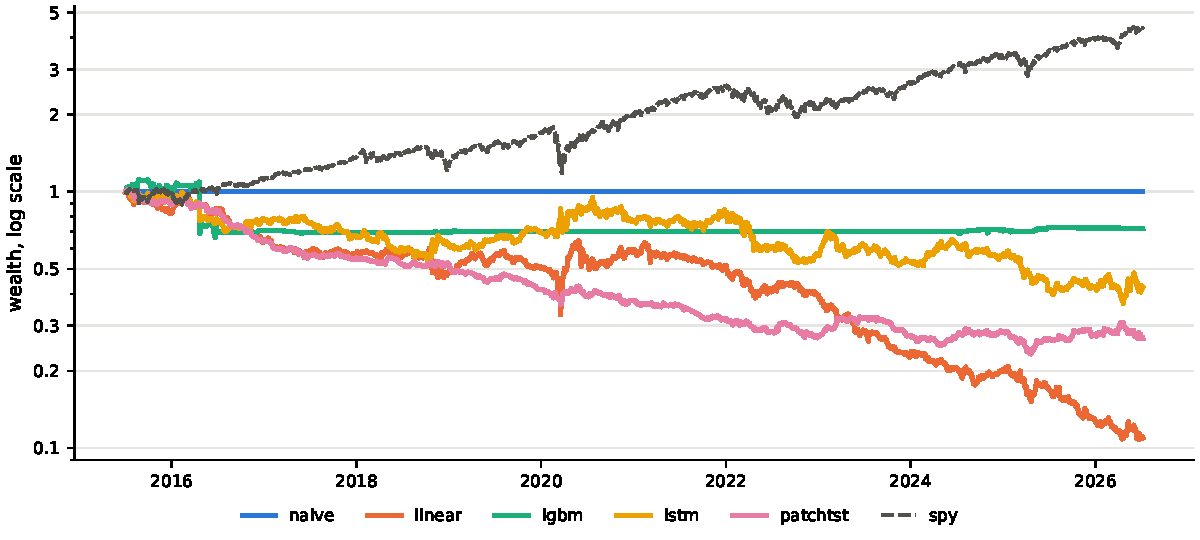
\includegraphics[width=\textwidth]{figures/wealth_dir.pdf}
\caption{Net wealth of the direction-based books on a log scale, seeds averaged into one daily return series per model, against buy-and-hold SPY (dashed).}
\label{fig:wealth_dir}
\end{figure}

\begin{figure}[H]
\centering
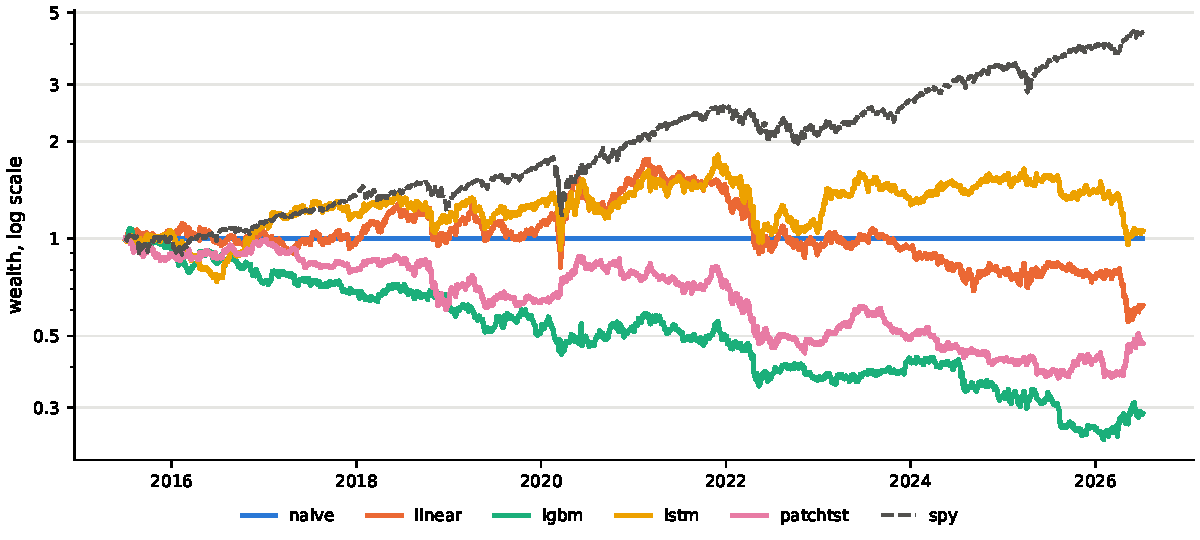
\includegraphics[width=\textwidth]{figures/wealth_rank.pdf}
\caption{Net wealth of the rank-based books on a log scale, as Figure~\ref{fig:wealth_dir}.}
\label{fig:wealth_rank}
\end{figure}

Tables~\ref{tab:bt_dir} and \ref{tab:bt_rank} and Figures~\ref{fig:wealth_dir} and \ref{fig:wealth_rank} report the backtest. No strategy makes money net of costs. The best net result is the LSTM traded on its rank predictions, which ends the eleven years roughly flat ($-0.1\%\pm5.4\%$ a year across seeds, Sharpe $+0.11\pm0.23$, $t=+0.4$); every other book loses between 3 and 18 per cent a year, and the two that are statistically distinguishable from zero (logistic regression and PatchTST on direction, $t=-2.7$ and $-2.3$) lose. Buy-and-hold SPY over the same days returns $14.2\%$ a year with a Sharpe ratio of $0.83$ and $t=3.0$.

Turnover explains the result. A book that is rebuilt every five days from a prediction with almost no persistence turns over between 98 and 147 units of capital a year, so at 10 basis points per unit traded the cost drag is between 10 and 15 percentage points of annual return. The break-even cost at which a strategy's net return would be zero is, to first order, its gross annual return divided by its annual turnover: about 10 basis points for the LSTM on rank ($10.2\%/98$), 7 for ridge on rank, 4 for PatchTST on rank, and 1 to 3 for every direction-based book. Only the LSTM's rank book is priced at roughly its break-even, which is why it ends flat; the others are below it. The gross Sharpe ratios tell the same story from the other side: the highest, $0.51\pm0.22$ for the LSTM on rank, is below SPY's $0.83$, and PatchTST's gross Sharpe on rank ($0.29\pm0.39$) has a seed range that spans zero. LightGBM's direction book trades 6.5 units of capital a year because its predictions are constant in most folds; the few folds in which it trades lose. The naive books never trade and are shown for completeness.

\subsection{Seed stability}

\begin{table}[H]
\centering\small
\caption{Pooled primary metric and net Sharpe ratio by seed for the two neural models.}
\label{tab:seeds}
\begin{tabular}{llrrrrr}
\toprule
Model & Seed & Vol RMSE & Dir accuracy & Rank IC & Dir net Sharpe & Rank net Sharpe \\
\midrule
LSTM & 0 & $0.5222$ & $0.5138$ & $0.0132$ & $-0.21$ & $-0.15$ \\
LSTM & 1 & $0.5324$ & $0.5138$ & $0.0218$ & $-0.37$ & $+0.22$ \\
LSTM & 2 & $0.5255$ & $0.5057$ & $0.0218$ & $-0.14$ & $+0.28$ \\
PatchTST & 0 & $0.5082$ & $0.5377$ & $-0.0056$ & $-0.51$ & $-0.29$ \\
PatchTST & 1 & $0.5119$ & $0.5372$ & $0.0133$ & $-0.51$ & $+0.23$ \\
PatchTST & 2 & $0.5160$ & $0.5263$ & $-0.0120$ & $-1.06$ & $-0.67$ \\
\bottomrule
\end{tabular}

\end{table}

Table~\ref{tab:seeds} shows the three seeds of each neural model individually. On volatility the three seeds of each model lie within $0.01$ RMSE of one another, an order of magnitude less than the gap to the random walk and less than the gap between the LSTM and the other models, so the comparison with LightGBM and ridge is not sensitive to initialisation. On direction the seeds agree on being below the base rate. On rank the seed spread is larger than the mean for PatchTST (IC between $-0.01$ and $+0.02$) and the net Sharpe ratios of both models span zero; the single LSTM seed with a positive net Sharpe of $+0.28$ would, if reported alone, suggest a marginally profitable strategy, which illustrates why a multi-seed protocol is necessary for this class of claim.

\subsection{Computational cost}

The three baselines fit all 33 task-folds in under a minute in total. The LSTM fits in 8 to 15 seconds each. PatchTST fits took a median of 250 seconds on the direction task, 330 seconds on volatility and 500 seconds on rank (the rank fits ran more epochs before early stopping), and the 99 PatchTST fits account for about nine of the ten hours of a full run on an Apple M5 laptop. Each fit's predictions are cached to disk so that an interrupted run resumes at the fit that was in flight.

\section{Discussion}\label{sec:discussion}

\paragraph{Why the transformer does not help.} Three features of the problem make it unfavourable to a sequence encoder of this kind. First, the hand-built features already summarise the lookback window: lagged returns at six horizons, realised volatility at three, momentum oscillators and a drawdown statistic are the quantities a patch encoder would have to rediscover from raw channels, and the linear and tree models receive them directly. The sequence models receive the same 43 channels as a window and must learn, from about 55{,}000 windows per fold with high noise, which of the $64\times43$ inputs matter; on the volatility target, where the answer is ``the recent realised-volatility channels, shrunk'', PatchTST learns it well enough to match LightGBM, and on the two return targets, where there may be nothing to learn, it fits noise. Second, channel independence is the right inductive bias for the benchmarks on which PatchTST was developed but it discards cross-channel structure at the encoder level; only the final linear mixer combines channels, so interactions such as ``high VIX and negative momentum'' are available to LightGBM but not to the encoder. Third, the effective sample is small. Five-day returns on 46 correlated names over five years provide far fewer independent observations than the row count suggests, and the regularisation that early stopping provides (most fits stopped by the second or third epoch) is coarse.

\paragraph{The volatility result in context.} That ridge regression wins on volatility is consistent with the long record of simple, heavily parameterised-by-hand models in this literature \citep{corsi2009simple,hansen2005forecast}. The random-walk naive is a weak benchmark for a five-day realised measure; the unconditional training mean would score an RMSE of about $0.62$, still well above every model, and a HAR-style regression on the three realised-volatility features alone would likely capture most of ridge's gain. The practically relevant finding is that the ordering ridge $<$ LightGBM $\approx$ PatchTST $<$ LSTM $\ll$ naive is stable across seeds and is only disturbed by the 2020 regime break, in which the simplest model degrades least.

\paragraph{The return results in context.} The direction and rank results are consistent with the weak-form efficiency of large liquid US names at a weekly horizon once technical information alone is used \citep{fama1970efficient,welch2008comprehensive}. The small rank IC of the LSTM and ridge is of the order reported for short-term reversal in individual stocks \citep{jegadeesh1990evidence}, and like that anomaly it does not survive realistic costs at a weekly rebalance \citep{novymarx2016taxonomy}. We stress that the backtest is a diagnostic of the forecasts, not a trading strategy: no attempt was made to lower turnover through signal smoothing, longer holding or trade netting, any of which would be the first step for a practitioner and all of which would be dominated by first finding a stronger signal.

\paragraph{What would change the conclusion.} The harness isolates three dimensions along which a transformer could still earn its cost: more cross-sectional breadth (thousands of names rather than 46, as in \citet{gu2020empirical}), information beyond price and volume (fundamentals, order flow, text), and a longer horizon at which the signal-to-noise ratio of the target improves. Each can be tested by changing a configuration file and a feature function without touching the evaluation protocol.

\section{Limitations}\label{sec:limitations}

\begin{itemize}[leftmargin=1.4em]
\item \textbf{Survivorship.} The universe is a hindsight selection of today's large caps (Section~\ref{sec:data}); absolute levels of the base rate, of SPY and of every book are inflated.
\item \textbf{Single vendor, adjusted prices.} Yahoo Finance adjusted closes are the only source; corporate actions are handled by the vendor's adjustment factors and were not audited.
\item \textbf{Fixed hyperparameters.} The neural architectures and training schedule were fixed before the test folds were scored and were not tuned on validation loss beyond early stopping. A larger search might improve PatchTST on volatility; it is unlikely to create a direction or rank signal where early stopping found none at epoch one.
\item \textbf{No refit on train plus validation.} Models are tested with the weights obtained on the training block alone; refitting on train and validation with the selected hyperparameters is common practice and would add six months of data to each fit.
\item \textbf{Asymmetric lookback convention.} Test windows may reach back into the validation block (Section~\ref{sec:walkforward}); this is live-trading information and not leakage, but it is a choice.
\item \textbf{Backtest simplifications.} Daily reset to target weights, no intra-period drift, no risk-free rate or short rebate, no borrow constraints, and a flat cost per unit traded. Drawdowns are on a book with two dollars of gross exposure per dollar of capital.
\item \textbf{No multiple-comparison correction.} Fifteen model-task pairs are tested against two baselines. Every significant result favours the simpler model, so a correction would not change the conclusions, but the marginal rank IC $t$-statistic of $2.1$ for the LSTM should be read with that in mind \citep{harvey2016cross}.
\item \textbf{One hardware path.} Neural results were produced on an Apple GPU; bitwise reproducibility was observed on that device but is not guaranteed by the framework across devices.
\end{itemize}

\section{Conclusion}\label{sec:conclusion}

Under a walk-forward protocol in which every channel of leakage is closed and tested, with identical information for every model and formal tests of predictive accuracy against two baselines, a PatchTST encoder adds no predictive value for five-day volatility, direction or cross-sectional rank of liquid US equities. It matches gradient-boosted trees on volatility, where a ridge regression on the same features is better than both, and it is null on the two return targets, where every model is null. Net of ten basis points per side, no forecast in the set can be traded at a profit through a five-day long/short book. The result is a defensible null rather than an absence of effort: three seeds, eleven out-of-sample years, two baselines and a costed backtest all point the same way. The harness is released so that the next architecture, feature set or universe can be evaluated under the same rules.

\bibliographystyle{plainnat}
\bibliography{refs}

\appendix

\section{Universe}\label{app:universe}

The \metantickers{} tradable names, by Yahoo Finance ticker: SPY, AAPL, MSFT, AMZN, GOOGL, NVDA, AMD, INTC, CSCO, IBM, QCOM, ADBE, NFLX, DIS, CMCSA, HD, NKE, MCD, JPM, BAC, WFC, GS, MS, AXP, JNJ, PFE, MRK, UNH, ABT, AMGN, LLY, XOM, CVX, PG, KO, PEP, WMT, COST, BA, CAT, HON, GE, UNP, UPS, T, VZ


\section{Per-fold results}\label{app:folds}

\begin{table}[H]
\centering\small
\caption{Volatility RMSE by test fold, seed-averaged; the last row pools all test samples.}
\begin{tabular}{llrrrrr}
\toprule
Fold & Test start & Naive & Ridge / logistic & LightGBM & LSTM & PatchTST \\
\midrule
0 & 2015-07 & $0.6330$ & $0.4925$ & $0.4949$ & $0.5531$ & $0.4923$ \\
1 & 2016-07 & $0.7135$ & $0.5478$ & $0.5524$ & $0.5826$ & $0.5510$ \\
2 & 2017-07 & $0.6557$ & $0.5083$ & $0.5191$ & $0.5308$ & $0.5160$ \\
3 & 2018-07 & $0.6320$ & $0.4790$ & $0.4927$ & $0.5183$ & $0.4952$ \\
4 & 2019-07 & $0.6158$ & $0.5433$ & $0.6044$ & $0.6115$ & $0.6408$ \\
5 & 2020-07 & $0.6071$ & $0.4753$ & $0.4834$ & $0.5239$ & $0.5106$ \\
6 & 2021-07 & $0.5983$ & $0.4682$ & $0.4694$ & $0.4802$ & $0.4739$ \\
7 & 2022-07 & $0.5851$ & $0.4475$ & $0.4703$ & $0.4482$ & $0.4432$ \\
8 & 2023-07 & $0.6461$ & $0.4885$ & $0.4986$ & $0.4965$ & $0.4820$ \\
9 & 2024-07 & $0.6617$ & $0.5066$ & $0.5179$ & $0.5285$ & $0.5093$ \\
10 & 2025-07 & $0.6261$ & $0.4878$ & $0.4879$ & $0.4982$ & $0.4908$ \\
\midrule Pooled & all & $0.6349$ & $0.4958$ & $0.5098$ & $0.5267$ & $0.5120$ \\
\bottomrule
\end{tabular}

\end{table}

\begin{table}[H]
\centering\small
\caption{Direction accuracy by test fold, seed-averaged.}
\begin{tabular}{llrrrrr}
\toprule
Fold & Test start & Naive & Ridge / logistic & LightGBM & LSTM & PatchTST \\
\midrule
0 & 2015-07 & $0.5519$ & $0.5520$ & $0.5519$ & $0.5088$ & $0.5449$ \\
1 & 2016-07 & $0.5679$ & $0.5669$ & $0.5679$ & $0.5244$ & $0.5543$ \\
2 & 2017-07 & $0.5831$ & $0.5804$ & $0.5831$ & $0.4723$ & $0.5396$ \\
3 & 2018-07 & $0.5879$ & $0.5879$ & $0.5879$ & $0.4769$ & $0.5548$ \\
4 & 2019-07 & $0.5589$ & $0.5591$ & $0.5589$ & $0.5691$ & $0.5282$ \\
5 & 2020-07 & $0.5822$ & $0.5822$ & $0.5822$ & $0.5794$ & $0.5487$ \\
6 & 2021-07 & $0.5078$ & $0.5078$ & $0.5078$ & $0.4841$ & $0.4953$ \\
7 & 2022-07 & $0.5371$ & $0.5371$ & $0.5371$ & $0.5080$ & $0.5373$ \\
8 & 2023-07 & $0.5593$ & $0.5288$ & $0.5593$ & $0.5048$ & $0.5262$ \\
9 & 2024-07 & $0.5528$ & $0.5528$ & $0.5528$ & $0.4603$ & $0.5128$ \\
10 & 2025-07 & $0.5312$ & $0.5258$ & $0.5312$ & $0.5332$ & $0.5304$ \\
\midrule Pooled & all & $0.5562$ & $0.5526$ & $0.5562$ & $0.5111$ & $0.5337$ \\
\bottomrule
\end{tabular}

\end{table}

\begin{table}[H]
\centering\small
\caption{Rank IC by test fold, seed-averaged.}
\begin{tabular}{llrrrrr}
\toprule
Fold & Test start & Naive & Ridge / logistic & LightGBM & LSTM & PatchTST \\
\midrule
0 & 2015-07 & $0.0000$ & $0.0040$ & $-0.0361$ & $-0.0550$ & $-0.0051$ \\
1 & 2016-07 & $0.0000$ & $0.0297$ & $0.0360$ & $0.0866$ & $-0.0019$ \\
2 & 2017-07 & $0.0000$ & $0.0426$ & $0.0155$ & $0.0513$ & $0.0155$ \\
3 & 2018-07 & $0.0000$ & $-0.0001$ & $-0.0120$ & $-0.0144$ & $-0.0241$ \\
4 & 2019-07 & $0.0000$ & $0.0211$ & $-0.0318$ & $0.0150$ & $0.0055$ \\
5 & 2020-07 & $0.0000$ & $0.0390$ & $0.0435$ & $0.0549$ & $0.0089$ \\
6 & 2021-07 & $0.0000$ & $-0.0532$ & $-0.0194$ & $-0.0472$ & $-0.0511$ \\
7 & 2022-07 & $0.0000$ & $0.0153$ & $0.0004$ & $0.0698$ & $0.0536$ \\
8 & 2023-07 & $0.0000$ & $-0.0119$ & $0.0284$ & $0.0134$ & $-0.0283$ \\
9 & 2024-07 & $0.0000$ & $0.0441$ & $0.0049$ & $0.0293$ & $-0.0067$ \\
10 & 2025-07 & $0.0000$ & $0.0244$ & $0.0229$ & $0.0049$ & $0.0179$ \\
\midrule Pooled & all & $0.0000$ & $0.0141$ & $0.0047$ & $0.0189$ & $-0.0014$ \\
\bottomrule
\end{tabular}

\end{table}

\section{Reproduction}\label{app:repro}

The experiment is the configuration \texttt{configs/exp02.yaml} of the \texttt{stockbench} repository at revision \texttt{\metasha}; its SHA-256 configuration hash is \texttt{\metaconfighash}. Software: Python \metavpython, NumPy \metavnumpy, pandas \metavpandas, scikit-learn \metavscikitlearn, LightGBM \metavlightgbm, statsmodels \metavstatsmodels, PyTorch \metavtorch, yfinance \metavyfinance. The run is reproduced with
\begin{verbatim}
uv sync
sh scripts/fix_macos_venv.sh          # macOS only
uv run pytest                         # leakage and unit tests, 39 cases
uv run python -m stockbench run --config configs/exp02.yaml
uv run python scripts/build_paper.py  # tables, figures and this document
\end{verbatim}
The run writes \texttt{reports/exp02/}: per-sample predictions, the metric and Diebold--Mariano tables, the backtest tables and daily return series, the figures, a Markdown summary and a manifest with the configuration, git revision, data range and library versions. Each of the 297 fits is cached as one Parquet file under \texttt{reports/exp02/cache/}, keyed by task, fold, model, seed and a hash of the fit-relevant configuration, so an interrupted run resumes and a change to the evaluation code alone re-renders the report in under a minute. Every table and figure in this document is generated from those files by \texttt{scripts/build\_paper.py}; no number is typed by hand.

\end{document}
